%%%%%%%%%%%%%%%%%%%%%%%%%%%%%%%%%%%%%%%% DECLARATION %%%%%%%%%%%%%%%%%%%%%%%%%%%%%%%%%%%%%%%%
\documentclass[12pt,english]{article}
\usepackage{graphicx}
\usepackage[T1]{fontenc}
%\usepackage{babel}
\usepackage[utf8]{inputenc} % set coding
%\usepackage{czech}
\usepackage[legalpaper, portrait, margin=0.8in]{geometry}
\usepackage{fixltx2e}
%\usepackage[czech]{babel}
\usepackage{hyperref}
\usepackage{textgreek}
\usepackage{textcomp}
\usepackage{adjustbox}
\usepackage{float}
\usepackage{tabto}
\usepackage{amsmath}
\newcommand\mytab{\tab \hspace{10mm}}
\usepackage{xcolor}
\usepackage{csvsimple}
\usepackage{multirow}
\usepackage{pdflscape}
\usepackage{pdfpages}
\usepackage{amsmath}
\usepackage{vaucanson-g}
\usepackage{amsfonts} 
\usepackage{blkarray}
\usepackage{listings}
\usepackage{xcolor}
\usepackage{multicol}

% Define a custom style for JSON
\lstdefinestyle{jsonstyle}{
  basicstyle=\ttfamily\small,
  commentstyle=\color{gray},
  keywordstyle=\color{blue},
  numberstyle=\tiny\color{red},
  stringstyle=\color{olive},
  tabsize=2,
  showstringspaces=false,
  breaklines=true
}

\author{Pavel Šesták, Samuel Janek}

\date{03.10.2023}  


%%%%%%%%%%%%%%%%%%%%%%%%%%%%%%%%%%%%%%%% TITLE PAGE %%%%%%%%%%%%%%%%%%%%%%%%%%%%%%%%%%%%%%%%
\begin{document}
  \begin{titlepage}
		\begin{center}
			%\textsc{\LARGE Vysoké Učení Technické v Brně} \\[0.5cm]
			%{\LARGE Fakulta informačních technologií}

			\begin{figure}
				\center
\includegraphics[scale=0.3]{images/logo.png}
			\end{figure}

			\vspace{3cm}

			\textsc{\LARGE Advanced Database Systems } \\[0.5cm]
			\textsc{\LARGE 2023/2024} \\[3.5cm]

			\textbf{\LARGE Command Query Responsibility Segregation} \\[1cm]
			\vspace{3cm}
		    \vspace{3cm}
		    
		    {\Large Samuel Janek (xjanek03)} \\[0.5cm]
		    {\Large Pavel Šesták (xsesta07)} \\[0.5cm]
		    
			
			\vspace{3cm}
                
		    \textsc{}{\LARGE Brno, \today}

		\end{center}
	\end{titlepage}

%%%%%%%%%%%%%%%%%%%%%%%%%%%%%%%%%%%%%%%% CONTENT TABLE %%%%%%%%%%%%%%%%%%%%%%%%%%%%%%%%%%%%%%%%
\begin{center}
	\tableofcontents %content generate
	\listoffigures
    \listoftables
	\clearpage %end of page
\end{center}


  
%%%%%%%%%%%%%%%%%%%%%%%%%%%%%%%%%%%%%%%% SECTIONS       %%%%%%%%%%%%%%%%%%%%%%%%%%%%%%%%%%%%%%%%
 
\section{Introduction}
 Command Query Responsibility Segregation is a general architectural pattern that separates the two main responsibilities in a system: commands (Commands) and queries (Queries).

\subsection*{Command service}
On this side, the requests for writing and editing data are processed. The complete business logic of the application, including input data validation, occurs here. To keep the application data consistent, the data is written to relational database that allows transactional processing and meets ACID properties.
 
\subsection*{Query service}
This side of the application is used to query the data, that are stored here in a more optimal form for reading than in the relational database. Data is typically reordered and denormalized to eliminate JOIN operations and speed up querying. Thus, NoSQL databases are typically used. The synchronization of these NoSQL databases is based on events that are retrieved from the Command service. Typically, there is some delay between writing data to the relational database and writing it to the NoSQL database.

\section{Specification}
In this section, we will briefly introduce the project and discuss the operations in our system. Since this is an e-shop, we will assume that the frequency of reading data greatly exceeds the frequency of writing and modification.


\subsection{Custom assignment}
In the context of the assignment, let us consider a virtual marketplace similar to the portals \href{www.amazon.com}{Amazon} or \href{www.aliexpress.com}{Aliexpress}. Within the portal, both vendors and customers can register. Customer can display the goods offered by vendors. The vendors are grouped into categories according to the products they currently offer on the e-shop. The customer can browse the marketplace and add goods to the cart. He can then order the goods and create a review on the items he has ordered. The review can be viewed on the item itself and on the vendor's profile.

\newpage
\subsection{System sequence diagram}
This diagram models the most common scenario of the customer's use of the system. 
\begin{figure}[hp]
    \centering
    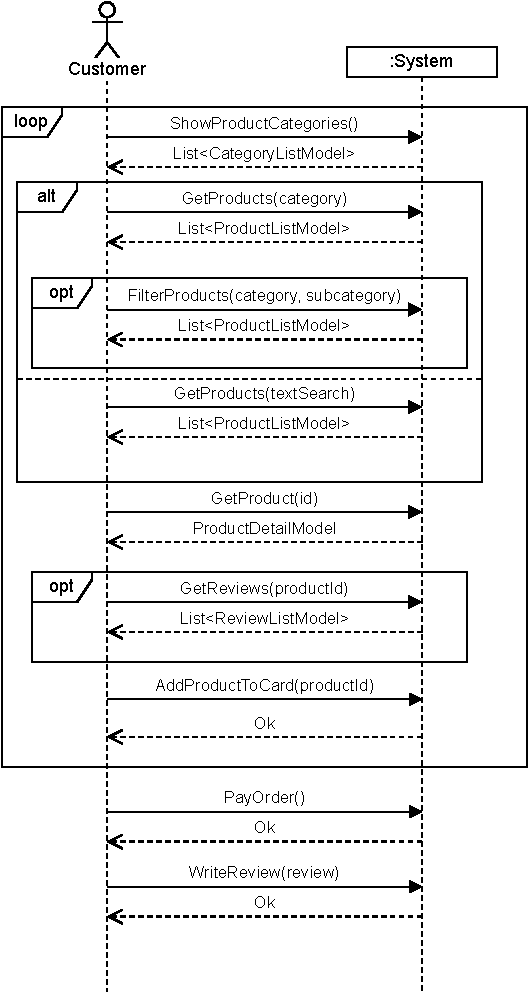
\includegraphics[scale=1.3]{images/systemSequenceDiagram_buy.pdf}
    \caption{System sequence diagram}
    \label{fig:my_label}
\end{figure}

\newpage
\subsection{Commands}
In this section we describe the commands over each identified entity within the system.

\begin{multicols}{2}

\noindent \textbf{Vendor}
\begin{itemize}
    \item Create
    \item Update
    \item SoftDelete
\end{itemize}
\textbf{Customer}
\begin{itemize}
    \item Create
    \item Update
    \item Anonymize (We can't delete the customer due to their order history, but we must remove their GDPR-sensitive data.)
\end{itemize}
\columnbreak
\textbf{Product}
\begin{itemize}
    \item Create
    \item SoftDelete
\end{itemize}
\textbf{Order}
\begin{itemize}
    \item Create
    \item AddProductToCart
    \item Pay
\end{itemize}
\textbf{Review}
\begin{itemize}
    \item Create
\end{itemize}
\textbf{Address}
\begin{itemize}
    \item Create
    \item Update
    \item Delete
\end{itemize}

\end{multicols}


\subsection{Queries}

In this section, we describe queries used in our system. Within the structure, we specify the expected use of the endpoint and the data structure in JSON format, where square brackets are used to denote collections and curly brackets for objects. The attribute is in the format <name:datatype>. Most queries are available to everyone, including unregistered users, as forcing registration to view products could negatively affect conversion rates (A measure of how many visitors become clients). \\

\noindent\textbf{Get customers}\\
Usage: Admin panel\\
Role: Manager, Administrator
\begin{lstlisting}[style=jsonstyle]
[
    {
        id: bigint,
        fullName: string,
        email: string,
        phoneNumber: string
    }
]
\end{lstlisting}

\noindent\textbf{Get vendors}\\
Usage: Admin panel\\
Role: Manager, Administrator
\begin{lstlisting}[style=jsonstyle]
[
    {
        id: bigint,
        name: string
    }
]
\end{lstlisting}

\newpage
\noindent\textbf{Get customer detail by email}\\
Usage: Customer profile page\\
Role: User (can see only his/her own account details), Manager, Administrator
\begin{lstlisting}[style=jsonstyle]
[
    {
        id: email as string,
        firstName: string,
        lastName: string
        phoneNumber: string,
        addresses: [
            {
                country: string,
                zipCode: string,
                city: string,
                street: string,
                houseNumber: string
            }
        ]
    }
]
\end{lstlisting}

\noindent\textbf{Get vendor detail by id}\\
Usage: Vendor profile page
\begin{lstlisting}[style=jsonstyle]
[
    {
        id: bigint,
        name: string,
        category: [string],
        address: {
            country: string,
            zipCode: string,
            city: string,
            street: string,
            houseNumber: string
        }
    }
]
\end{lstlisting}

\noindent\textbf{Get products}\\
Usage: Landing page
\begin{lstlisting}[style=jsonstyle]
[
    {
        id: bigint,
        title: string,
        price: double,
        rating: 5,
        vendor: {
            id: bigint,
            name: string
        }
    }
]
\end{lstlisting}

\newpage
\noindent\textbf{Get products by category}\\
Usage: Landing page
\begin{lstlisting}[style=jsonstyle]
[
    {
        id: category as string,
        products: [
            {
                id: bigint,
                title: string,
                price: double,
                rating: int,
                vendor: {
                    id: bigint,
                    name: string
                }
            }
        ]
    }
]
\end{lstlisting}

\noindent\textbf{Get products by subcategory}\\
Usage: Landing page
\begin{lstlisting}[style=jsonstyle]
[
    {
        id: subcategory as string,
        products: [
            {
                id: bigint,
                title: string,
                price: double,
                rating: 5,
                vendor: {
                    id: bigint,
                    name: string
                }
            }
        ]
    }
]
\end{lstlisting}

\noindent\textbf{Get product reviews}\\
Usage: Product detail page
\begin{lstlisting}[style=jsonstyle]
[
    {
        rating: double,
        text: string
    }
]
\end{lstlisting}

\noindent\textbf{Get product detail by id}\\
Usage: Product detail page
\begin{lstlisting}[style=jsonstyle]
{
    id: bigint,
    title: string,
    description: string,
    piecesInStock: number,
    price: number,
    rating: number,
    vendor: {
        id: bigint,
        name: string
    },
    categories: [string],
    subcategories: [string]
}
\end{lstlisting}

\newpage
\noindent\textbf{Get orders for user}\\
Usage: Customer profile
\begin{lstlisting}[style=jsonstyle]
[
  {
    id: email as string,
    orders: [
        {
            id: bigint
            status: enum,
            price: number,
            created: timestamp,
            updated: timestamp,            
        }
    ],
    
  }
]
\end{lstlisting}

\noindent\textbf{Get order detail by id}\\
Usage: Customer profile
\begin{lstlisting}[style=jsonstyle]
{
    id: bigint,
    status: enum,
    price: number,
    address: {
        country: string,
        zipCode: string,
        city: string,
        street: string,
        houseNumber: string,
    },
    created: datetime,
    updated: datetime,
    products: [
        {
            id: bigint,
            title: string,
            description: string,
            price: number,
            vendor: {
                id: bigint,
                name: string
            }
        }
    ]  
}
\end{lstlisting}

\noindent\textbf{Get categories}\\
Usage: Landing page
\begin{lstlisting}[style=jsonstyle]
[
    {
        id: categoryname as string,
        description: string
        subcategories: [
            {
                name: string,
                description: string
            }
        ]
    }
]
\end{lstlisting}

\newpage

\section{Design}
In this section, we summarize the information from the specification and formalize it into models based on which the system will be further implemented. 

\subsection{High-level Component diagram}
This diagram models the distribution of services and their interconnection.
\begin{figure}[hp]
    \centering
    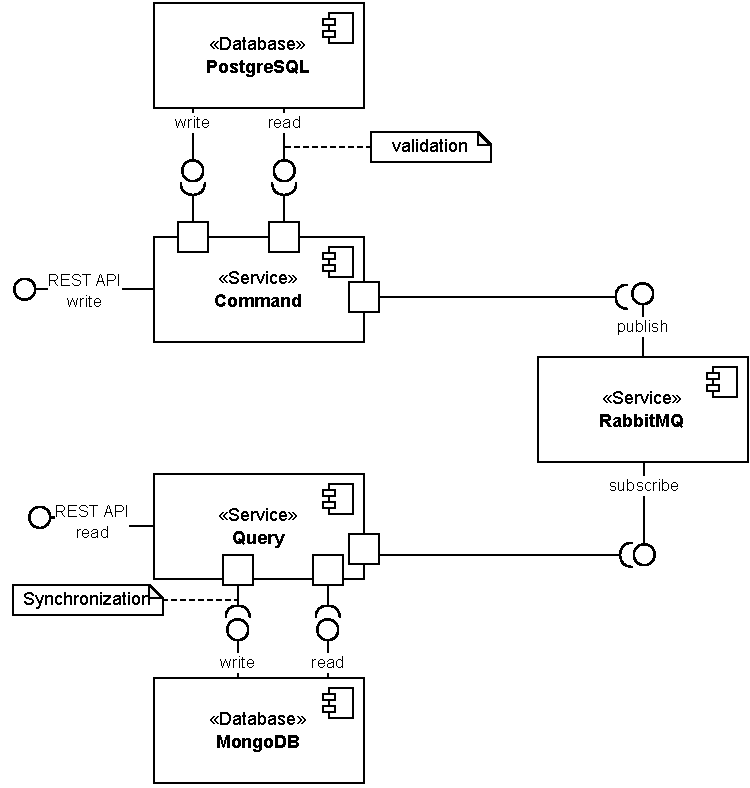
\includegraphics[scale=1.1]{images/componentDiagram.pdf}
    \caption{High-level Component diagram}
    \label{fig:my_label}
\end{figure}
\newpage
\subsection{Detail Component diagram}
The detailed component diagram gives us a closer look at the system architecture. Where we are already dealing with the link between the individual packages and parts of the system at the code level.
\begin{figure}[hp]
    \centering
    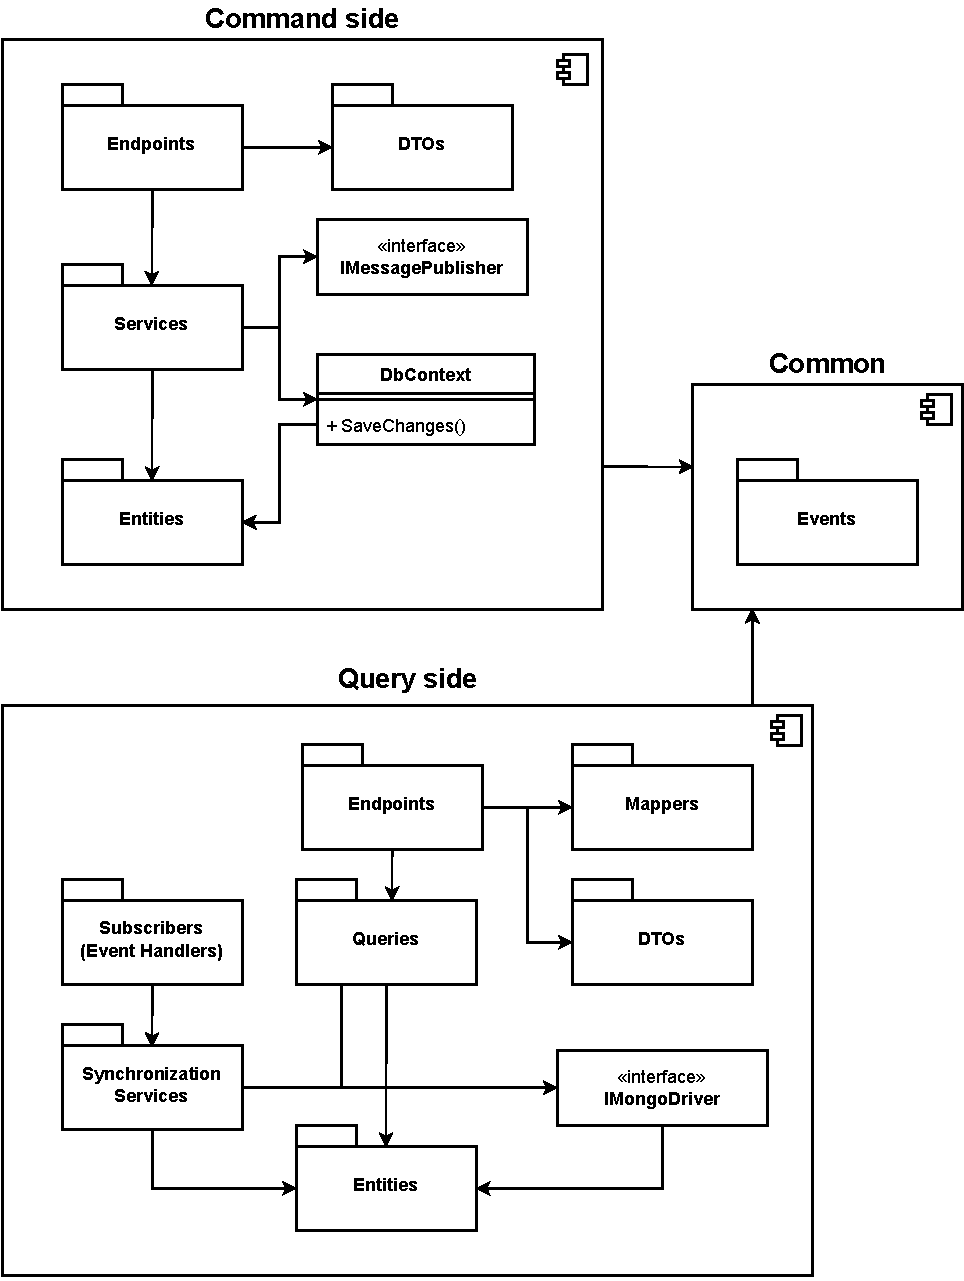
\includegraphics[scale=0.8]{images/pdb-system-diagram.pdf}
    \caption{Detail Component diagram}
    \label{fig:my_label}
\end{figure}

\subsection{Synchronising data stores}
For synchronization between the relational and NoSQL database we chose the message broker Rabbit.MQ, within which we create a channel for each entity in the system. The message will contain the type of operation (create, edit, delete) and the necessary data to perform the NoSQL database update. Rabbit.MQ supports data persistence, so if the read service goes down, it will be delivered when it comes back up. Thus, on the relational database side, if the database is edited, the appropriate message is sent to the appropriate channel. Subsequently, on the read side, there will be a service for each channel that will provide the read service from the channel and edit any necessary collections so that the collections reflect the actual state in the relational database.


\newpage
\subsection{E-R Diagram}
This diagram represents specific tables and data layouts within a relational database.
\begin{figure}[hp]
    \centering
    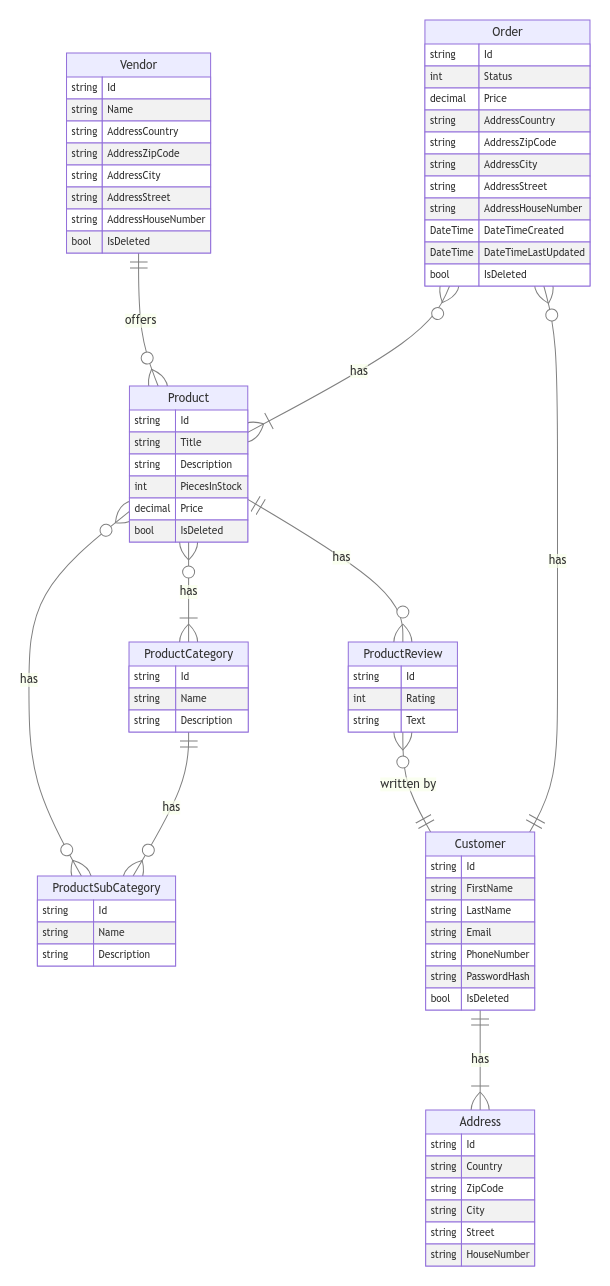
\includegraphics[scale=.45]{images/erd.png}
    \caption{ER - Diagram}
    \label{fig:my_label}
\end{figure}


\newpage

\subsection{MongoDB}
MongoDB is a document database system. It stores data in collections, where each collection consists of documents. It stores data in BSON (binary JSON) format. Collections are schema-less, which is useful for storing sparse data or for adding attributes dynamically. Proper database design is crucial for efficient searching, where we can use index support for more complex searches. MongoDB is also found in modern web stacks as the main persistent storage due to its support for transactional locking, which provides us with database consistency. MongoDB supports distributed deployments and the associated data replication and horizontal database scaling support.


\subsubsection{Data validity period}
The validity of data in the NoSQL database will directly correlate with the validity in the relational database, since the NoSQL database is primarily used here to streamline queries and reduce JOIN operations over relational data.

\subsubsection{Scalability}
Scalability is a key feature of MongoDb, without which we could not talk about it as a modern data store. It is a key feature for large and fast growing applications that require high availability. There are two main approaches to scaling the system. For large systems, it is advisable to combine these two approaches.\\

\noindent\textbf{Horizontal scaling (Sharding)}\\
With horizontal scaling, we spread the load across multiple nodes so that each node contains only a portion of the data. The distribution between nodes is done using a suitable sharding key. Then the query is sent to the router and it already knows the network tology and where to look for the answer to the query according to the provided sharding key.\\

\noindent\textbf{Vertical scaling}\\
Vertical scaling consists of increasing the hardware resources of a given node.

\subsubsection{Definition of collections}
In this section we will define the individual database collections and discuss how often the data will be accessed and why we chose the following layout for this application.\\

\noindent\textbf{Collection of vendors}\\
The collection contains information about vendors. We have embedded categories into the collection so it can be used when a customer views a vendor's profile. In the case of a large number of vendors, we can use a hashed shard key for distribution via the vendor name attribute.
\begin{lstlisting}[style=jsonstyle]
[
    {
        _id: 1,
        name: "Vendor XYZ",
        category: ["Toys", "Pets"],
        address: {
            country: "The Czech Republic",
            zipCode: "561 64",
            city: "Jablonne Nad Orlici",
            street: "Lesni",
            houseNumber": "280"
        }
    }
]
\end{lstlisting}

\newpage
\noindent\textbf{Collection of customers}\\
Unlike the vendor table, we can expect a larger volume of data and faster data creation. We will use email as id, since this attribute must be unique. Since we won't need the address itself without the user we will get rid of one join and put the collection of addresses into the customer object. In case of a large number of customers, we can use a hashed shard key for distribution via the customer's email.
\begin{lstlisting}[style=jsonstyle]
[
    {
        _id: "email@gmail.com",
        firstName: "Adam",
        lastName: "Johnson",
        phoneNumber: "00420123123123",
        addresses: [
            {
                _id: 1,
                country: "The Czech Republic",
                zipCode: "262 42",
                city: "Rozmital Pod Tremsinem",
                street: "U medvidku",
                houseNumber: "1563"
            }
        ]
    }
]
\end{lstlisting}

\noindent\textbf{Collection of products}\\
We expect this collection to contain a large amount of data. Since we expect significantly more reads than writes, we have embedded vendor, categories and subcategories into collection. There is also total rating calculated based on the reviews of this product. In the case of a large number of products, we can use a hashed shard key over the product name for distribution, allowing for quick searches by name. An index would be created on the vendor name to efficiently display the products of that vendor.
\begin{lstlisting}[style=jsonstyle]
[
    {
        _id: 1,
        title: "Rat killer",
        description: "Poison for rats",
        piecesInStock: 1,
        price: 45.99,
        rating: 5,
        vendor: {
            _id: 1,
            name: "Extreminators",
        },
        categories: [
            {
                "name": "Pests"
            }
        ],
        subcategories: [
            {
                "name": "Poisons"
            }
        ]
    }
]
\end{lstlisting}

\newpage
\noindent\textbf{Collection of orders}\\
The order collection will be used to display the details of a given order from the customer's profile. Furthermore, the collection will be used to display the list of orders of the given user. For this purpose, we will create an index on the customer id. In the case of a large number of orders, we can use a hashed shard key for distribution through the customer, which will guarantee that all orders of one customer will be on just one node.
\begin{lstlisting}[style=jsonstyle]
[
    {
        _id: 1,
        customerId: 1,
        status: "paid",
        price: 49.90,
        address: {
            country: "Czech Republic",
            zipCode: "612 00",
            city: "Brno",
            street: "Bozetechova",
            houseNumber: "2/1"
        },
        created: "2023-10-16T15:30:00Z",
        updated: "2023-10-17T15:30:00Z",
        isDeleted: "false"
        products: [
            {
                _id: 1,
                title: "Rat killer",
                description: "Poison for rats",
                price: 45.99,
                vendor: {
                    _id: 1,
                    name: "Extreminators",
                },
            },  
        ]
        
    }
]
\end{lstlisting}

\noindent\textbf{Collection of reviews}\\
The review collection will contain an index to the product id, as we will primarily want to calculate reviews of specified product. In the case of a large number of reviews, we can use a hashed shard key to distribute them across the product, guaranteeing that all reviews of a single product will be on a single node.
\begin{lstlisting}[style=jsonstyle]
[
    {
        _id: 1,
        productId: 1,
        rating: 5,
        text: "Very good product"
    }
]
\end{lstlisting}

\newpage
\noindent\textbf{Collection of products of category}\\
Collection of products grouped by category for quick loading of products in the product catalog on the client side. This collection was designed purely for performance optimization of reading products (we do not need to apply filtering). Vertical scaling is not anticipated to be required for this collection.
\begin{lstlisting}[style=jsonstyle]
[
    {
        _id: "CategoryName",
        products: [
            {
                _id: 1,
                title: "Rat killer",
                description: "Poison for rats",
                price: 45.99,
                rating: 4,
                vendor: {
                    _id: 1,
                    name: "Extreminators",
                },
            }
        ]
    }
]
\end{lstlisting}
\textbf{Collection of products of subcategory}
Collection of products grouped by subcategory of given category for quick loading of products in the product catalog on the client side. This collection was designed purely for performance optimization of reading products (we do not need to apply filtering). Vertical scaling is not anticipated to be required for this collection.
\begin{lstlisting}[style=jsonstyle]
[
    {
        _id: ("ParentCategory", "SubCategory"),
        products: [
            {
                _id: 1,
                title: "Rat killer",
                description: "Poison for rats",
                price: 45.99,
                rating: 4,
                vendor: {
                    _id: 1,
                    name: "Extreminators",
                },
            }
        ]
    }
]
\end{lstlisting}


\noindent\textbf{Collection of categories}\\
This collection will be used on the landing page to display available categories of the products. We will insert the subcategory information directly into the collection record. We expect this collection to be stable (basically without modifications). Vertical scaling is not anticipated to be required for this collection.
\begin{lstlisting}[style=jsonstyle]
[
    {
        _id: 1,
        categoryName: "name",
        description: "description of category",
        subCategories: [
            {
                _id: 2,
                categoryName: "name"
            }
        ]
    }
]
\end{lstlisting}


\section{Technologies}
The system will be implemented using ASP.NET Core framework. Both read and write services will be implemented as web API. Communication between services will be handled by message broker RabbitMQ. Individual services will run in docker containers and we will use docker compose for deployment. Postgres database has been chosen as the relational database and MongoDB will be used on the read side of the service due to its versatility.

\section{Deployment}
The application is ready to be deployed within the Docker runtime environment, which enables easy deployment without the need to deal with dependencies and ensures isolated running of individual applications. Each application, service, and database is deployed within its own container where the docker compose tool is used to orchestrate the containers. The structure of each container is shown in the deployment diagram. Thus, to start the system, it is only necessary to have the docker daemon installed and running, and to start the application using the \texttt{docker compose up} command from the root directory, which contains the \texttt{docker-compose.yml} file. The Write Service is available at \texttt{\url{http://127.0.0.1:5000}, \url{https://127.0.0.1:5001}} and the Read Service at \texttt{\url{http://127.0.0.1:5002}, \url{https://127.0.0.1:5003}}. Both applications have an interactive OpenApi specification, which is available at the \texttt{/swagger} endpoint. From the root Write Service folder you need to run the database migration using \texttt{dotnet ef database update}. For this you will need the dotnet command line tool and the Entity Framework Design package.

\begin{figure}[tbhp]
    \centering
    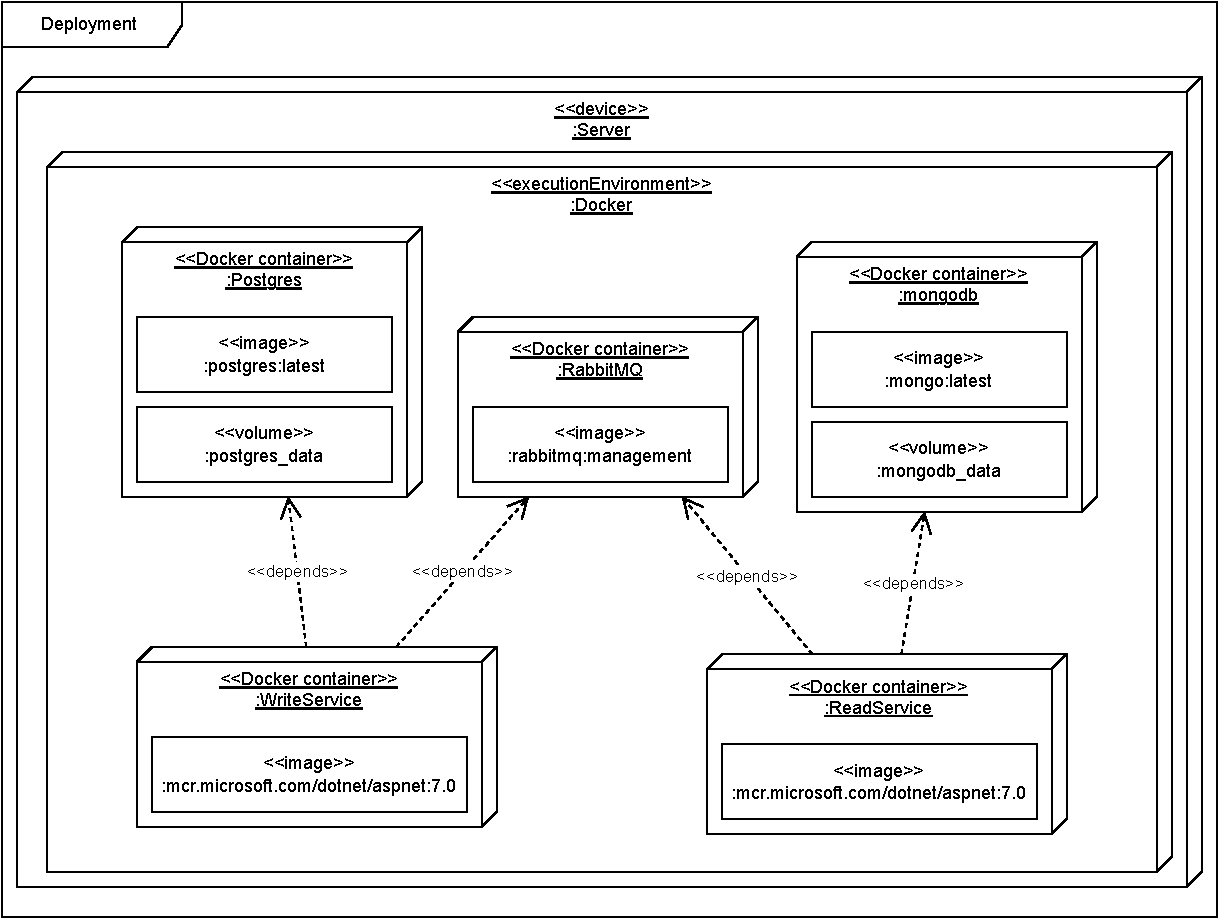
\includegraphics[scale=.8]{images/Deployment.pdf}
    \caption{Deployment Diagram}
\end{figure}

\section{Testing}
As part of the testing, automatic end-to-end tests were implemented using the \texttt{xunit} library. Applications are run inmemory using \texttt{WebApplicationFactory} and individual endpoints are called over them. Separate databases are used for testing. Each test is a scenario that involves creating or modifying data via the Write service, and then testing that the data has indeed been written to the Read service. It also tests whether the application adheres to consistency rules, such as making it impossible to order items that are already deleted or out of stock. 

\begin{figure}[tbhp]
    \centering
    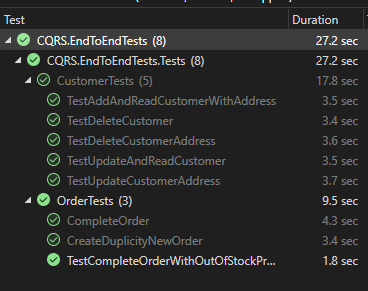
\includegraphics[scale=1.2]{images/automaticTests.PNG}
    \caption{Result of automatic tests}
\end{figure}
\newpage
The rest of the use cases were tested using the \texttt{Postman} application, which allows us to import the definition of individual services in the \texttt{OpenApi} format, which is made possible by the \texttt{Swagger} library. The Write Service call was manually tested and then whether the change was correctly propagated to the Read Service. Then it was manually verified using \texttt{pgAdmin} that the data was correctly modified within the relational database.

\begin{figure}[tbhp]
    \centering
    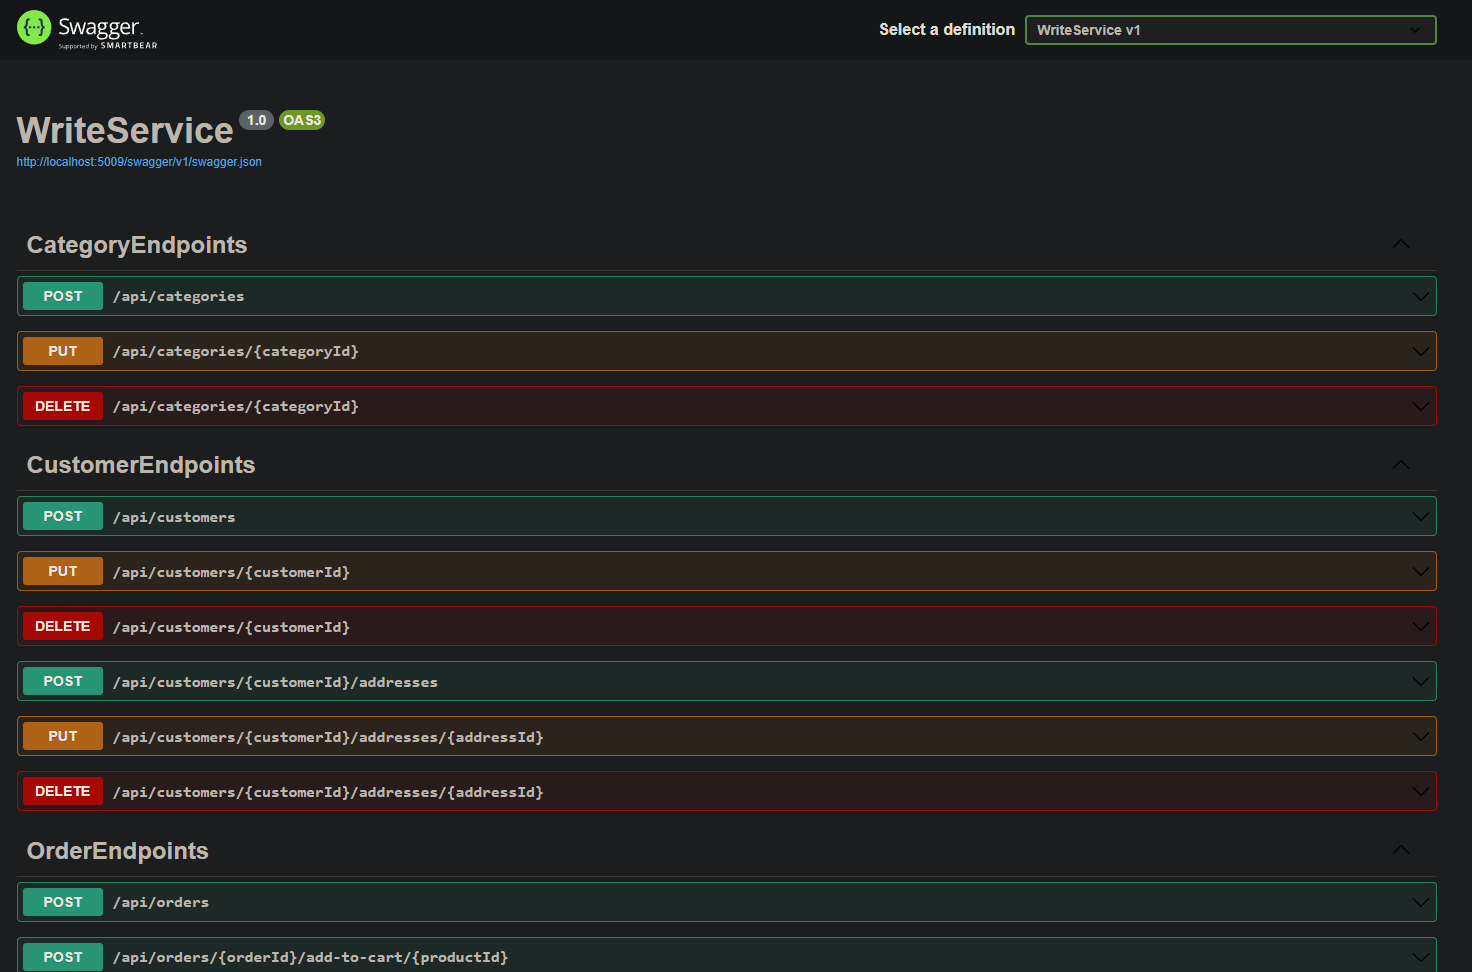
\includegraphics[scale=0.35]{images/swagger-write.PNG}
    \caption{OpenAPI Specification Write Service}
\end{figure}
\newpage
\begin{figure}[tbhp]
    \centering
    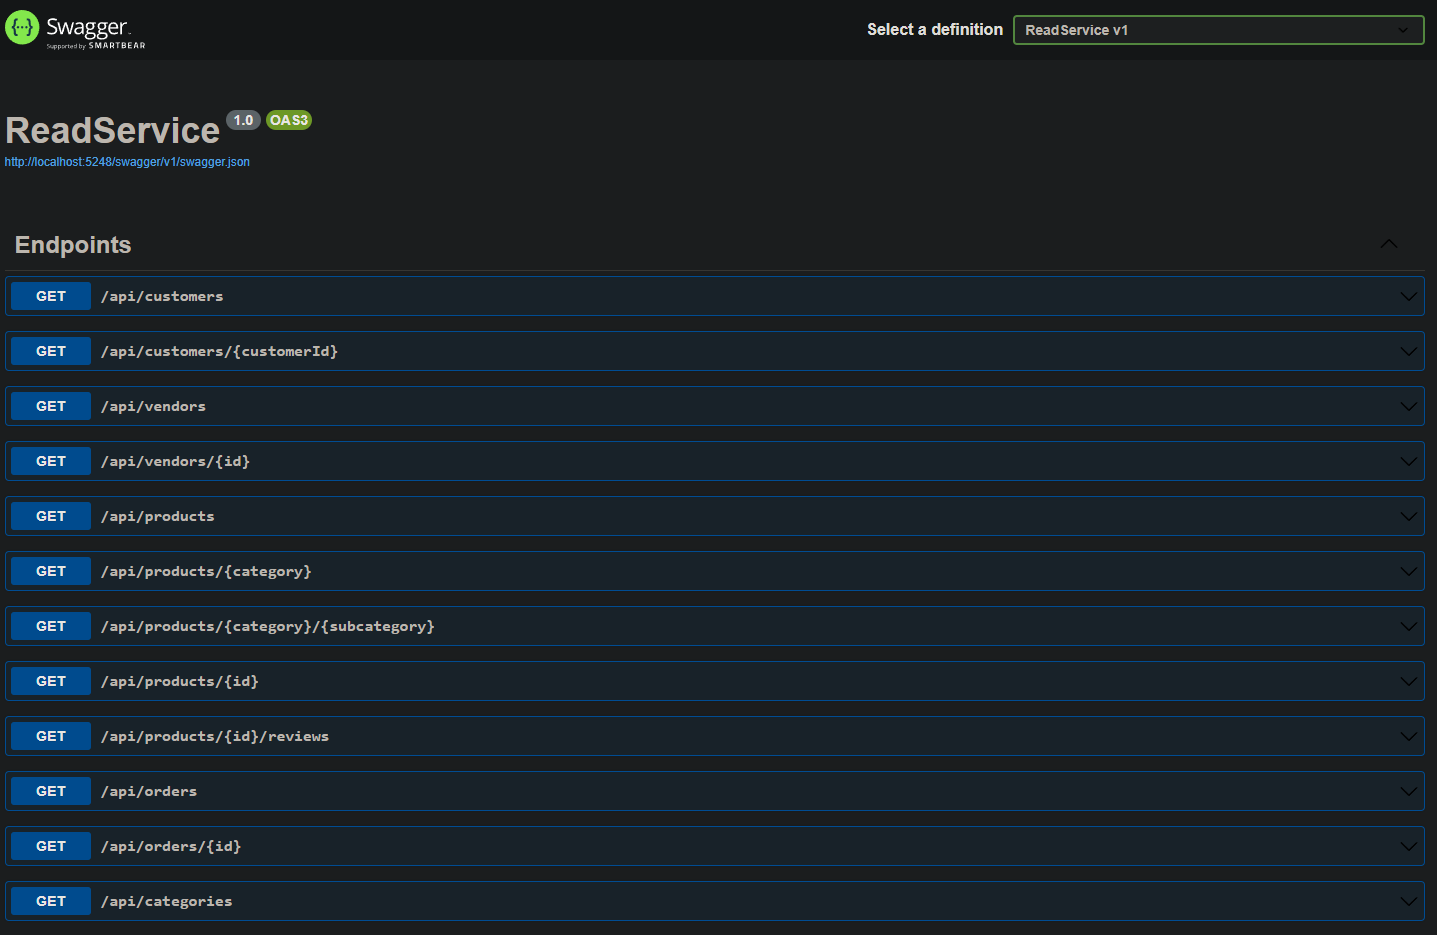
\includegraphics[scale=0.35]{images/swagger-read.PNG}
    \caption{OpenAPI Specification Read Service}
\end{figure}

\begin{figure}[tbhp]
    \centering
    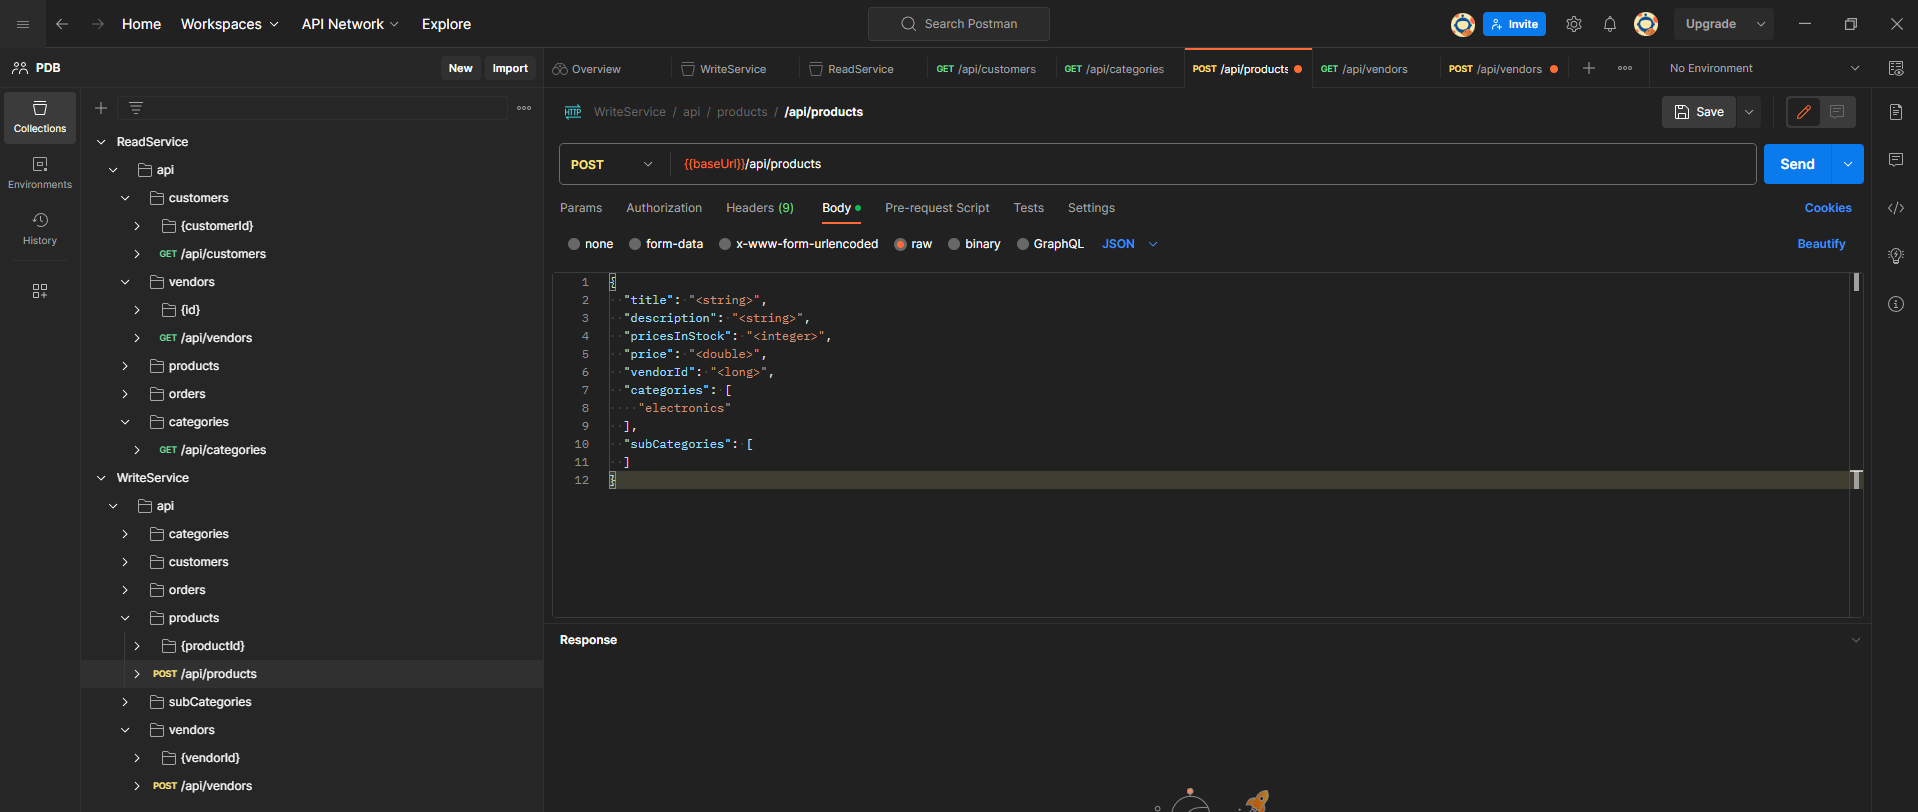
\includegraphics[scale=0.35]{images/postman.PNG}
    \caption{Postman workspace}
\end{figure}

\section{Conclusion}
The goal of this project was to test the principles associated with the implementation of the \texttt{CQRS} patter, so we did not consider user authentication and the absence of other functionalities that would certainly be needed to run a similar system in a real environment. However, the system as such works despite its limitations and both databases synchronize as expected.

%\newpage
%\bibliographystyle{czechiso}
%\bibliography{citace}
\end{document}
